\section{Randomiseret Min-Cut}
\subsection{Algoritmen}

Givet en sammenhængende ikke-orienteret graf $G = (V, E)$, da er et min-cut i $G$ en kantmængde $E'$ af minimal størrelse, så $(V, E \backslash E')$ er ikke-sammenhængende.\\

Algoritmen fungerer således:
\begin{itemize}
	\item Vælg kant $e$ uniformt i $E$
	\item Contract $e$ og fjern self-loops
	\item Gentag indtil antal knuder $|V'| = 2$
	\item Returner kantmængde mellem de to knuder
\end{itemize}

\begin{figure}[H]
	\begin{center}
		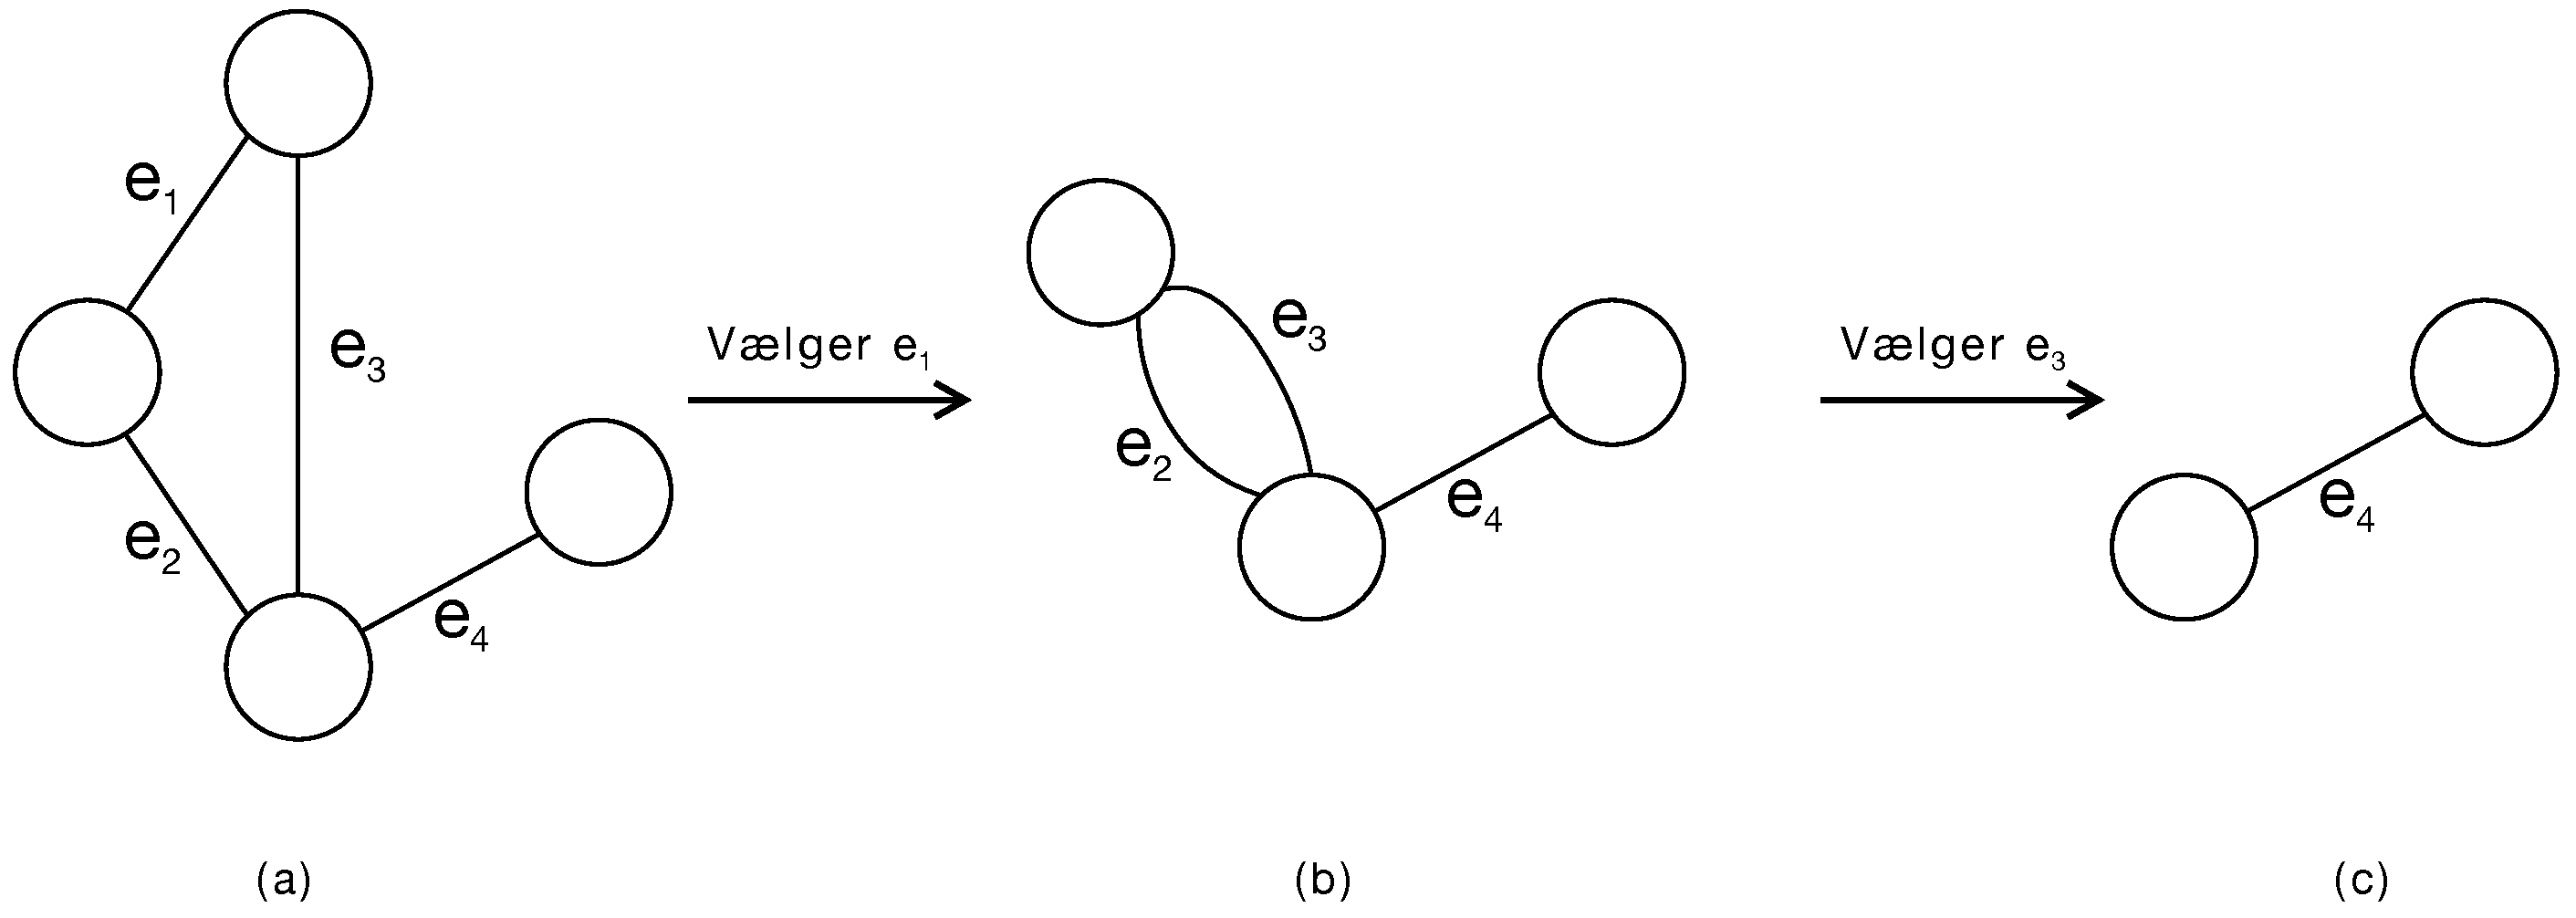
\includegraphics[width=\textwidth]{min-cut.pdf}
	\end{center}
	\caption{Eksempel på Min-Cut}
	\label{fig:min-cut}
\end{figure}

På \ref{fig:min-cut} fra (a) til (b) vælger vi $e_1$. Herved sker der en contraction. Fra (b) til (c) vælger vi $e_3$, hvorved der igen sker en contraction. Vi ser, at vi nu har et self-loop, så det fjerner vi. Nu er der kun to knuder tilbage, så algoritmen er færdig og vi returnerer kantmængden $\{e_4\}$.\\

\textbf{NB:} Bemærk at vi fra (b) til (c) potentielt godt kunne have valgt kant $e_4$, og herved ville vi ikke have fundet et min-cut.





\subsection{Analyse af sandsynligheden for at vælge en forkert kant}
Lad os nu definere et min-cut til $C$ og lade $k$ være antallet af kanter i $C$, $k = |C|$. Lad os derudover sige, at $n = |V|$. Og lad os indføre begrebet ''degree'' for hver knude, som beskriver antal kanter der rører knuden.\\


Betragt iteration $i$ hvor $1 \leq i \leq n-2$ (dette er netop det antal iterationer algoritmen vil gå igennem da vi stopper når der er to knuder tilbage).\\


Antag, at ingen af de kanter der løbende blev contracted i $G$ i iteration $1 \, .. \, i-1$  indgår i vores optimale løsning $C$, således vi ikke potentielt får en fejlagtig løsning.\\

Da der er $n$ knuder til at starte med og der fjernes én pr. contraction, så må der efter $i-1$ iterationer være $n-i+1$ knuder i $G$.\\

Da $k = |C|$ for et min-cut $C$, så må minimum cut-størrelsen i $G$ være $\geq k$. Derfor må der altså også som minimum være $k$ kanter der rører hver knude, så $G_{\text{min\_degree}} \geq k$.\\

Da vi havde, at der var $n-i+1$ knuder i $G$, og vi lige har vist at de alle minimum har degree $k$, så kan vi få et lower bound for antal kanter $|E|$ i $G$:
\begin{align}
|E| \geq \frac{(n-i+1)k}{2}
\end{align}

Her dividerer vi med 2, da vi tager højde for at enhver kant $e$ vil røre to knuder.\\

Således kan vi bestemme sandsynligheden for at en af kanterne i $C$ contractes i iteration $i$ til:
\begin{align}
\P[\text{En kant i $C$ contractes i iteration $i$}] = \frac{k}{|E|} \leq \frac{k}{\frac{1}{2}(n-i+1)k} = \frac{2}{n-i+1}
\end{align}
Dette gælder, da $k$ er antallet af kanter i $C$ og vi ønsker at finde sandsynligheden for at vi tilfældigt vælger en af disse kanter ud af alle kanter $|E|$.